%-----------------------------------------------------------------------------%
\chapter{ANALISIS DAN PERANCANGAN SISTEM}
%-----------------------------------------------------------------------------%
\vspace{4.5pt}

Pada bab ini menjelaskan analisis masalah yang diatasi, alur kerja dari perangkat lunak yang dikembangkan, arsitektur dan metode yang digunakan serta hasil evaluasi.\\

\section{Analisis Masalah}
Arsitektur ERP yang digunakan pada Odoo yaitu arsitektur monolitik, seperti yang sudah dijelaskan pada landasan teori. Arsitektur monolitik memiliki kelemahan dan permasalahan yang bisa diselesaikan dengan arsitektur \textit{microservice}.

Namun untuk melakukan perubahan arsitektur harus dilakukan dekomposisi, proses dekomposisi sendiri tidak mudah karena proses dekomposisi masih membutuhkan analisis secara manual dan untuk mengidentifikasi \textit{service} sulit karena banyaknya pendekatan dan pertimbangan.

Pada penelitian ini menggunakan pendekatan \textit{Hierarchical Clustering} untuk membantu menemukan \textit{service} yang tepat, di mana \textit{Hierarchical Clustering} memberikan rekomendasi bagaimana pengelompokan \textit{service} berdasarkan pemilihan partisi.

Proses dimulai dari melalukan analisis kode seperti \textit{Call Graph} yang dihasilkan dari kode aplikasi Odoo. Hasil analisis kode di ekstraksi menjadi matriks untuk dilakukan \textit{Hierarchical Clustering}. \textit{Linkage} yang digunakan dalam melakukan \textit{Hierarchical Clustering} yaitu \textit{single}, \textit{complete}, dan \textit{average}, kemudian  Partisi  dipilih melalui nilai secara struktural yaitu nilai \textit{coupling}  dan \textit{cohesion}. Hasil terbaik dari \textit{clustering} disampling untuk diimplementasikan menjadi \textit{service}, penelitian ini akan menggunakan strategi dengan pola \textit{strangle fig } dan \textit{branch by abstraction} untuk memecah kode di monolitik.

\section{Kerangka Pemikiran}
\begin{center}
	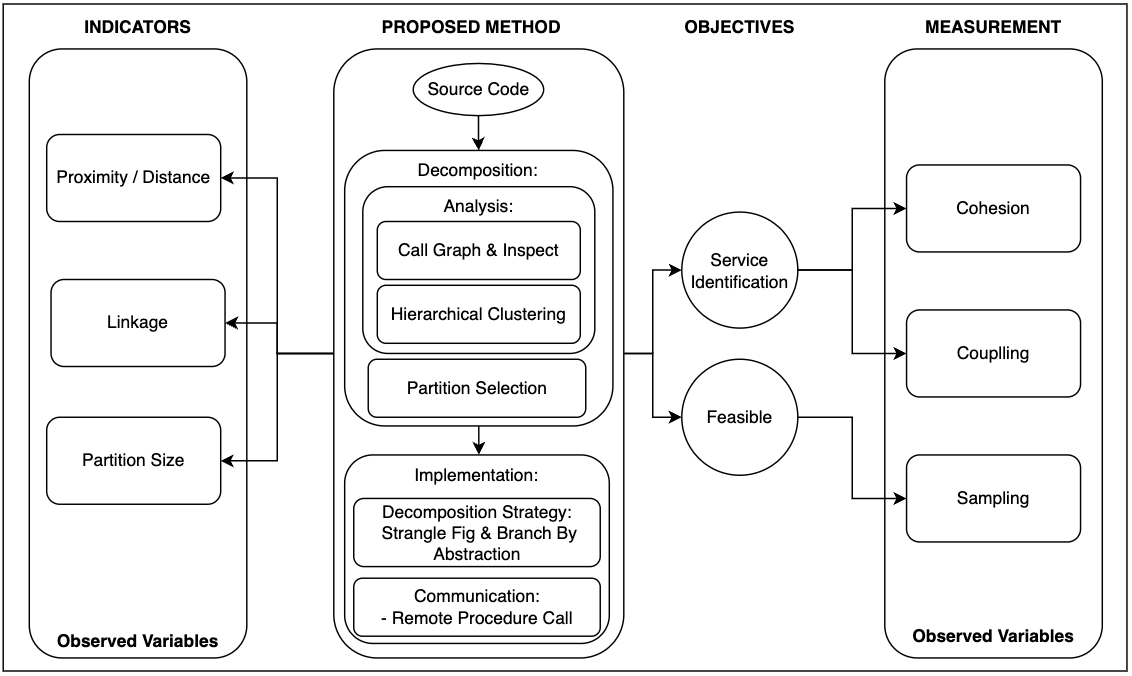
\includegraphics[width=14cm]{img/bab_3/KerangkaPemikiran.png}
	\captionof{figure}{Kerangka Pemikiran}
	\label{fig:kerangka_pemikiran}
\end{center}

Penelitian akan dimulai dengan menggunakan kode sumber aplikasi yang dibuat dengan monolitik. Kode sumber dilakukan proses dekomposisi yaitu dengan analisis seperti mencari objek beserta atributnya, untuk mencari keterhubungan lebih lanjut tentang objek maka dilakukan pencarian pada fungsi-fungsi sehingga terbentuklah \textit{call graph} yang menunjukkan bagaimana keterhubungan masing-masing objek di aplikasi.

Dari \textit{graph} yang sudah dibuat akan dilakukan pengelompokan dengan algoritma \textit{Hierarchical Clustering}. Pendekatan algoritma yang digunakan pada penelitian ini yaitu agglomerative, selain itu ditentukan cara menghitung kedekatan antara objek dan pemilihan algoritma \textit{Linkage}. Metode \textit{linkage} yaitu menentukan jarak atau kemiripan antara semua objek. Untuk menentukan jarak ini bisa dengan rata-rata, maximum, dan minimum. 

Pengelompokan dari \textit{Hierarchical Clustering} akan dipilih dengan mencari nilai \textit{cohesion} terendah dan  nilai \textit{coupling} tertinggi. Di mana \textit{coupling} mengevaluasi tingkat ketergantungan langsung dan tidak langsung antar objek. Semakin banyak dua objek menggunakan metode masing-masing semakin mereka menjadi satu kesatuan. Sedangkan  \textit{cohesion} akan mengevaluasi kekuatan interaksi antar objek. Biasanya, dua objek atau lebih menjadi interaktif jika metodenya menggunakan metodenya satu sama lain. Dengan membandingkan nilai  \textit{coupling}, \textit{cohesion}, \textit{linkage} dan ukuran partisi maka dapat diketahui kelompok service yang ideal.

Selain itu, untuk mengetahui apakah hasil \textit{clustering} relevan dan dapat diimplementasikan maka dilakukan sampling yang berjumlah 2 service dari kelompok service yang ideal. Untuk menerapkannya pemecahan dimulai dari pemecahan kode yang menggunakan strategi dekomposisi \textit{strangle fig } dan \textit{branch by abstraction}. Untuk metode komunikasinya antara \textit{service} yaitu dengan Remote Procedure Call(RPC) dan untuk mengelola datanya, setiap \textit{service} memiliki databasenya masing-masing.\\

\section{Urutan Proses Global}
\begin{center}
	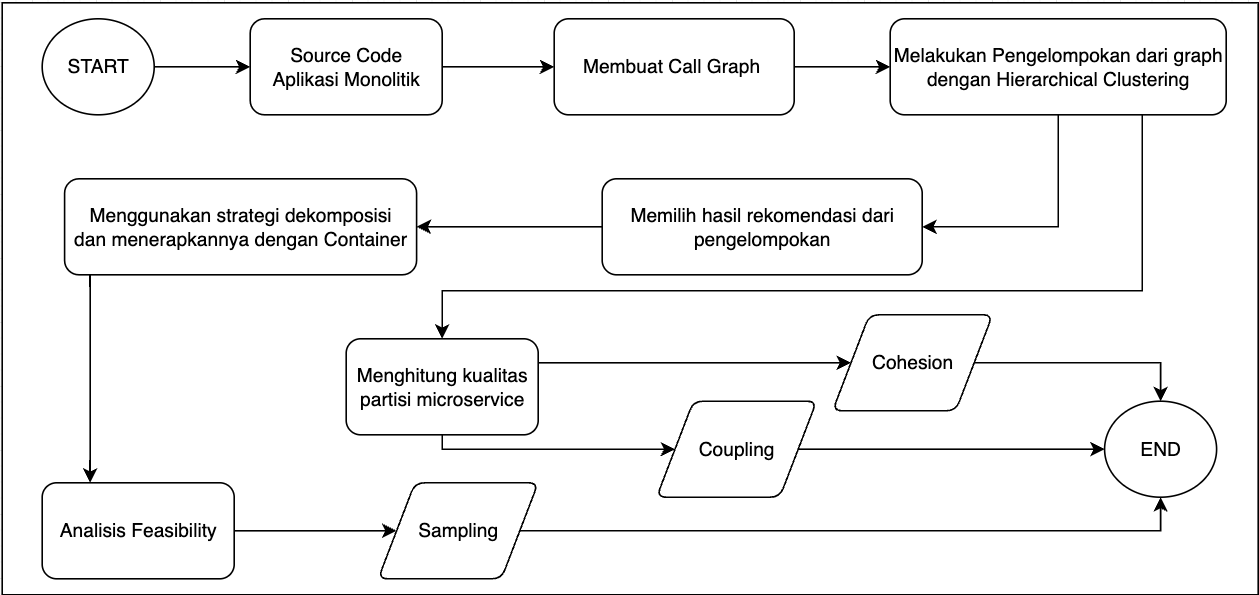
\includegraphics[width=14cm]{img/bab_3/FlowchartProsesGlobal.png}
	\captionof{figure}{Diagram Flowchart Proses Global }
	\label{fig:proses_Global}
\end{center}

\subsection{Proses Clustering}

\subsubsection{Pengambilan Source Code}
Aplikasi ERP Odoo merupakan aplikasi berlisensi open source, kode program dapat diunduh melalui situs repository Odoo. Pada tugas akhir ini menggunakan Odoo versi 16 dengan status pengujian lulus. Agar kode program dapat berjalan dengan lancar maka diperlukan proses installasi library, module dan Package yang digunakan dari file requirement.txt
\begin{center}
	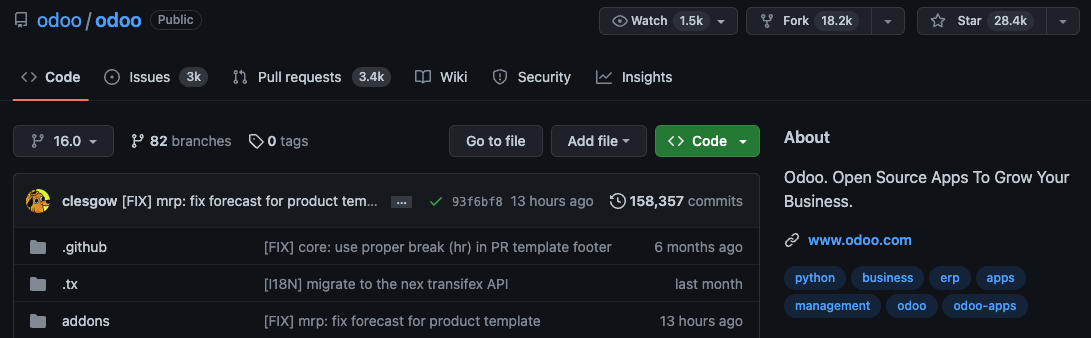
\includegraphics[width=14cm]{img/bab_3/github.png}
	\captionof{figure}{Source Code Aplikasi Odoo pada git repository}
	\label{fig:github_ss}
\end{center}

\subsubsection{Pembuatan \textit{Call Graph}}
Pada tugas akhir ini menggunakan tools PyCG untuk menghasilkan \textit{call graph} dalam bentuk format JSON. Terdapat target folder yang harus dianalisis oleh PyCG \textit{call graph} yaitu folder 'odoo/addons" atau package 'odoo.addons'. Pemilihan folder ini dikarenakan folder/package lainnya tidak memiliki hubungan mengenai proses bisnis. Untuk menghemat waktu pembuatan \textit{call graph} maka folder test dan l10n (localization) tidak dianalisis.  

\textit{Entry point} untuk \textit{tools} PyCG adalah semua file di target folder dengan ekstensi file .py serta ditentukan package yang ingin diolah menjadi \textit{call graph}. Proses eksekusi dilakukan melalui terminal. \textit{Call graph} yang dihasilkan berisi \textit{call} yang berasal dari file .py yang ditentukan sebelumnya dan semua module yang terhubungan dari target. Semua module ini bisa diluar dari target module apabila keterhubungan itu terus berlanjut. PyCG hanya bisa menghasilkan \textit{call graph} tanpa informasi mengenai jumlah pemanggilan dan urutan pemanggilan.

\begin{center}
	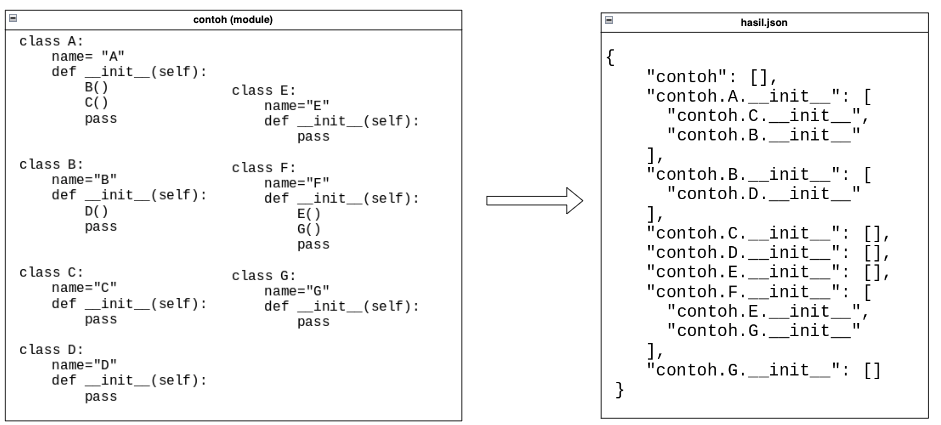
\includegraphics[width=13cm]{img/bab_3/soToCG.png}
	\captionof{figure}{Proses Pembuatan \textit{Call Graph} dengan PyCG}
	\label{contoh_json_pycg}
\end{center}

Proses ekstraksi json yang dihasilkan dari tools PyCG berupa file JSON yang dinamakan berdasarkan argrument yang diberikan sebelumnya seperti 'addons.json'. File JSON diubah menjadi \textit{graph} yang direpresentasikan dalam bentuk \textit{adjacency} list di Python.

\subsubsection{Ekstraksi Dependency Model}
Keterbatasannya informasi \textit{call graph} yang dihasilkan dari PyCG, sehingga tugas akhir ini menggunakan library Python yaitu 'inspect' untuk menganalisis objek secara run-time. Hal ini disebabkan Python adalah bahasa pemrogram dinamik di mana pengecekan tipe data dilakukan secara 'run-time'. Ekstrasi ini difokuskan pada module yang memiliki proses bisnis seperti module addons. Dari gambar 3.5 bisa diketahui penggunaan inspect bisa menemukan atribut apa saja dan nilainya dari atribut pada objek. 

\begin{center}
	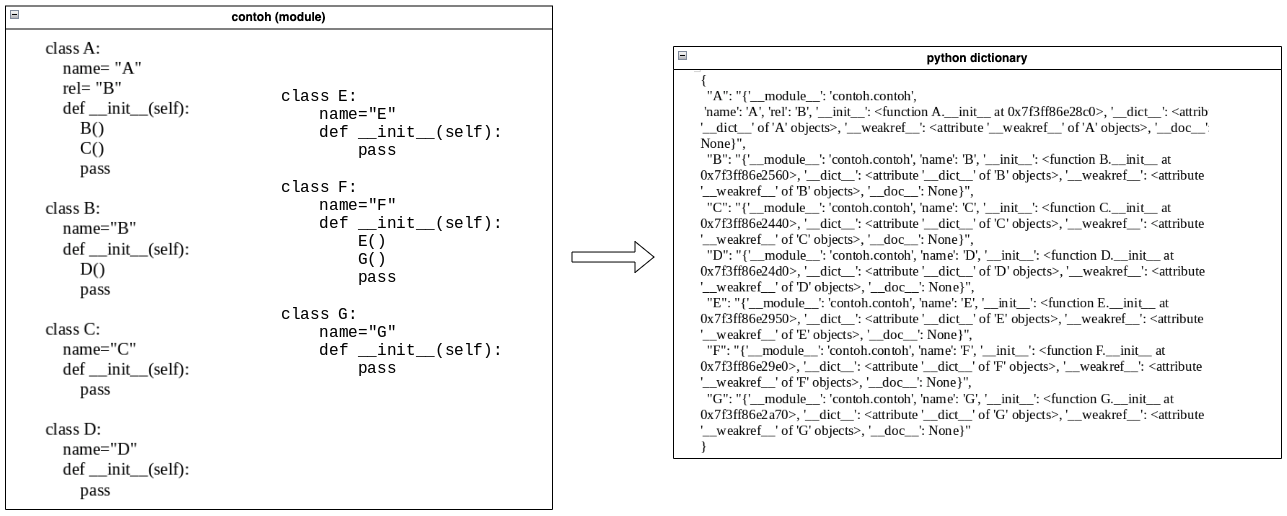
\includegraphics[width=13cm]{img/bab_3/inspectSample.png}
	\captionof{figure}{Penggunaan 'inspect' untuk melihat objek Python lebih mendalam}
	\label{contoh_inspectSample}
\end{center}

Object yang dianalisis yaitu \textit{class} yang merupakan turunan dari \textit{class} odoo.models.MetaModel, di mana \textit{class} MetaModel memiliki properti seperti  name, \_inherits , \_inherit, dan comodel\_name. Hasil ekstrasi dependency model digabungkan melalui nama module PyCG.

\subsubsection{Pengabungan dan Optimisasi Hasil Ekstraksi}
Graph yang dihasilkan dari proses ekstrasi dipisahkan antara module eksternal dan module internal. Module yang digunakan untuk pengelompokan adalah module internal, setiap \textit{call} yang dilakukan memiliki nama \textit{call} yang berupa gabungan antara nama fungsi / \textit{class} / module /file di kode program. PyCG tidak memberikan informasi apakah nama \textit{call} tersebut berupa tipe apa, untuk itu pengelompokan dilakukan secara campuran yaitu berdasarkan module dan file, yang dikelompokkan menjadi file hanya addons base.

Nama \textit{call} yang disatukan menjadi module adalah \textit{call} yang memiliki awalan(root) addons atau odoo/addons dan nama \textit{call} yang disatukan dengan file adalah nama \textit{call} selain addons. Call yang dikelompokkan memiliki nilai agregasi dari jumlah \textit{call}. Jumlah \textit{call} dapat digunakan sebagai weight yang dapat menunjukkan kekuatan antara \textit{call} satu sama lain, proses ini membentuk \textit{call} baru yang lebih ringkas dan relevan dalam bentuk \textit{graph}. 

Pada gambar \ref{fig:dg_al} dapat dilihat hasil dari graph yang dihasilkan dari contoh PyCG dan Inspect sebelumnya. Graph yang digunakan merupakan directed sehingga setiap pemanggilan berlaku untuk satu arah. Graph ini dapat diubah menjadi bentuk dictionary sebagai \textit{adjacency} list, tujuannya agar pengaksesan dan pencarian node lebih cepat dan mudah dilakukan. Setiap relasi memiliki jumlah berapa kali node lain dipanggil dari node tersebut.

\begin{center}
	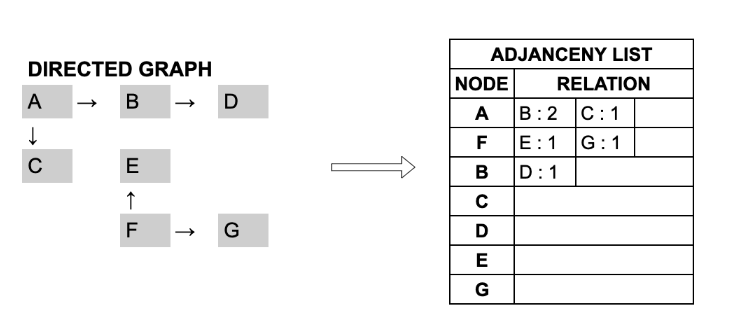
\includegraphics[width=13cm]{img/bab_3/dg_al.png}
	\captionof{figure}{Graph dan Adjanceny List}
	\label{fig:dg_al}
\end{center}

\subsubsection{Hierarchical Clustering}
Graph yang berbentuk \textit{Adjacency} list diubah menjadi \textit{adjacency} \textit{matrix}, proses normalisasi data dilakukan pada matriks. Tujuan normalisasi data agar nilai \textit{weight}(jumlah \textit{call}) dari relasi berkisar dari 1 hingga 0. Semakin banyak jumlah \textit{call} dilakukan maka nilai mendekati 1,kemudian matriks tersebut dibuat menjadi \textit{Distance} \textit{Matrix}, rumus jarak yang digunakan ada 2 yaitu Jaccard dan Struktural Similarity. Jaccard menghasilkan hasil yang bagus pada remodularisasi perangkat lunak dan Struktural Similarity digunakan untuk melihat kedekatan dari sisi intesitas panggilan antara module.

Berikut pada gambar \ref{fig:weight_normal_mat} dilakukan proses perubahan dari \textit{adjacency} list menjadi \textit{adjacency} \textit{matrix} yang memiliki bobot. Kemudian dilakukan normalisasi kolom, dimana setiap nilai dibandingkan dengan nilai maximum dan nilai minimum pada kolom yang sama. 

\begin{center}
	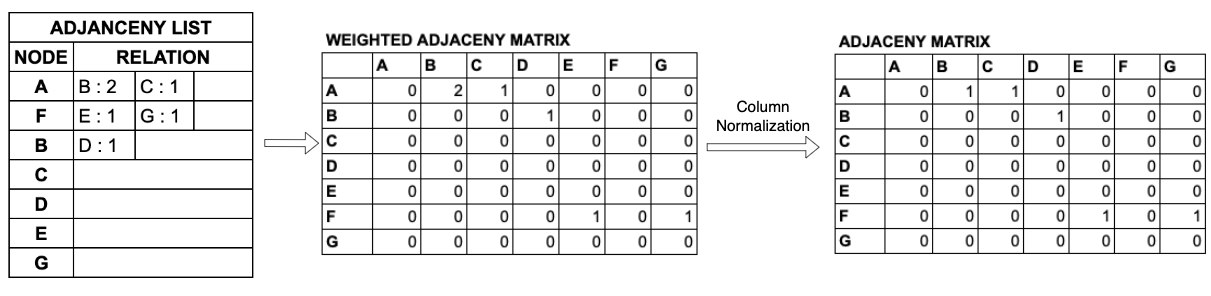
\includegraphics[width=14cm]{img/bab_3/weight_normal_mat.png}
	\captionof{figure}{Perubahan dari \textit{Adjacency} List menjadi \textit{Adjacency} \textit{Matrix}}
	\label{fig:weight_normal_mat}
\end{center}

Proses perhitungan jarak antara 2 objek dilakukan dari \textit{adjacency} \textit{matrix} dengan pola urutan berbentuk matriks segitiga bawah. Dengan ini perbandingan pertama kali dilakukan di baris ke-2(index=1) di kolom ke-1(index=0) dan berakhir pada baris ke-n(jumlah objek) di kolom  ke n-1. Pada contoh di \ref{fig:distance_detail} dijelaskan untuk perhitungan total jarak pada objek B dan A. Sebelum dilakukan perhitungan matriks terlebih dahulu sisi diagonal diberi nilai 1 untuk mengartikan bahwa objek memiliki hubungan dengan dirinya sendiri.  Perhitungan dimulai menghitung kimiripan jaccard, jaccard menghasilkan kemiripan dari jumlah interseksi dibagi jumlah union pada objek. Perhitungan selanjutnya Similarity Struktural menghitung dengan mempertimbangkan jumlah sisi panggilan kedua objek yaitu baris ke-1(index=0), baris ke-2(index=1) dan jumlah sisi panggilan keluar kedua objek yaitu kolom  ke-1(index=0) dan kolom ke-2(index=1). Hasil kemiripan Similarity Struktural dan Jaccard dirata-ratakan untuk menjadi nilai akhir kemiripan objek.

\begin{center}
	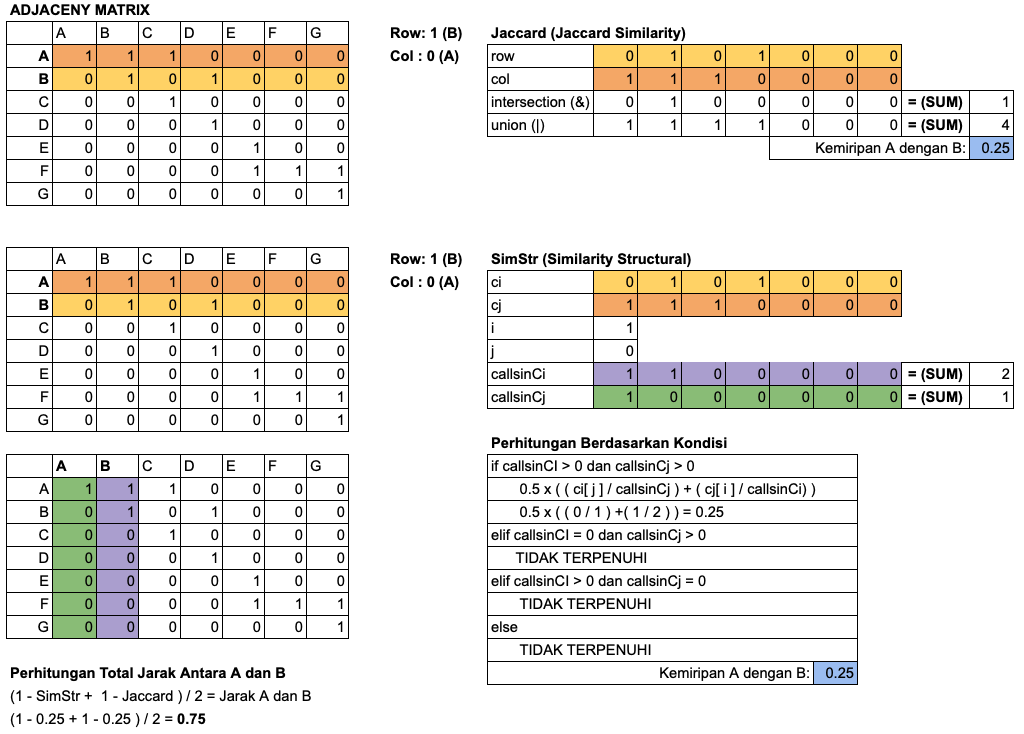
\includegraphics[width=14cm]{img/bab_3/distance_detail.png}
	\captionof{figure}{Perhitungan Jarak}
	\label{fig:distance_detail}
\end{center}

\begin{center}
	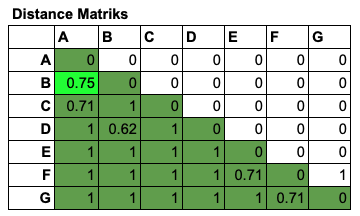
\includegraphics[width=7cm]{img/bab_3/distance_final.png}
	\captionof{figure}{Hasil Akhir Jarak}
	\label{fig:asd}
\end{center}

Distance \textit{Matrix} / Matriks kedekatan dapat dilihat nilai dengan ilustrasi Heatmap, di mana sumbu x dan y adalah semua module dan nilai kedekatannya dengan module lainnya. Semakin terang warna menunjukkan hubungan yang kuat antara module, perlu diketahui bahwa \textit{distance} \textit{matrix} merupakan matriks segitiga. Pada tugas akhir ini menggunakan library SciPy untuk melakukan proses \textit{clustering} yang memiliki fungsi \textit{Hierarchical Clustering}.

\begin{center}
	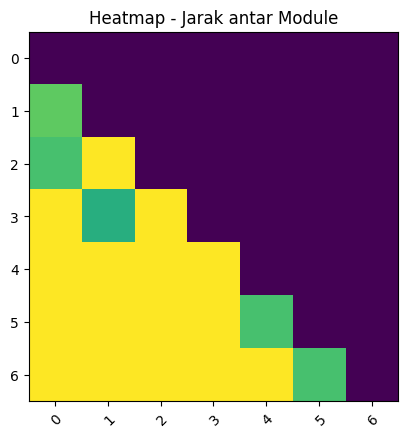
\includegraphics[width=7cm]{img/bab_3/heatmap.png}
	\captionof{figure}{Heatmap yang dihasilkan dari \textit{Distance} \textit{Matrix}}
	\label{fig:asd}
\end{center}

Pemilihan pengelompokan dengan hierarchical agglomerative \textit{clustering} dibandingkan Partition \textit{clustering} karena tidak mudah untuk mengetahui jumlah ideal \textit{cluster}. Untuk menentukan metode \textit{linkage} tugas akhir ini menggunakan \textit{single} linkage, \textit{average} \textit{linkage}, dan \textit{complete} linkage. Hasil dari masing-masing linkage dipilih jumlah partisi yang ideal untuk \textit{microservice}. Penggunaan \textit{single} linkage memiliki kecenderungan menghasilkan banyak partisi yang berisi modul sedikit tetapi ada satu partisi memiliki banyak module sedangkan \textit{complete} \textit{linkage} menghasilkan partisi yang memiliki jumlah modul yang sama dengan partisi lainnya. Untuk \textit{Average} linkage menghasilkan bentuk partisi di antara \textit{complete} linkage dan \textit{single} linkage.

Pada gambar \ref{fig:hc_detail_1} dijelaskan mengenai proses perhitungan \textit{Hierarchical Clustering} dengan \textit{distance} matriks yang sebelumnya sudah dihitung. Perhitungan \textit{Hierarchical Clustering} terdapat 5 bagian besar yaitu pertama memiliki objek pertama (urutan pertama), ke-2 mencari objek lainnya yang terdekat berdasarkan \textit{distance} \textit{matrix}, ke-3 mengabungkan objek yang terdekat dengan objek yang pertama dan membuat kelompok baru dari objek tersebut, ke-4 memperbaharui nilai jaraknya pada kelompok baru / partisi menggunakan \textit{linkage}. Penggunaan \textit{linkage} akan membandingkan 2 nilai objek yaitu dari nilai objek yang baru dan nilai objek yang sebelumnya (yang terdapat di \textit{distance} matriks) seperti min memilih nilai yang lebih rendah, \textit{complete} memilih nilai yang lebih tinggi, dan \textit{average} melakukan nilai rata-rata dari 2 nilai objek. Langkah terakhir bila sudah tidak ada objek tersisa maka perhitungan berhenti bila masih ada maka dilajukan kembali proses yang ke-2.

\begin{center}
	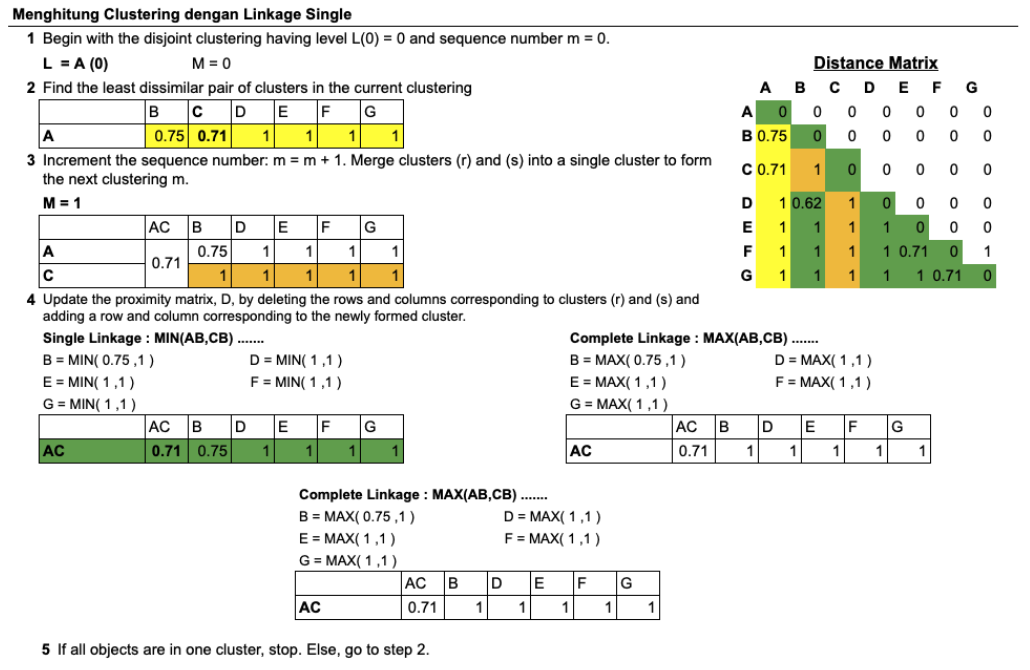
\includegraphics[width=14cm]{img/bab_3/hc_detail_1.png}
	\captionof{figure}{Proses Perhitungan \textit{Hierarchical Clustering}}
	\label{fig:hc_detail_1}
\end{center}

\begin{center}
	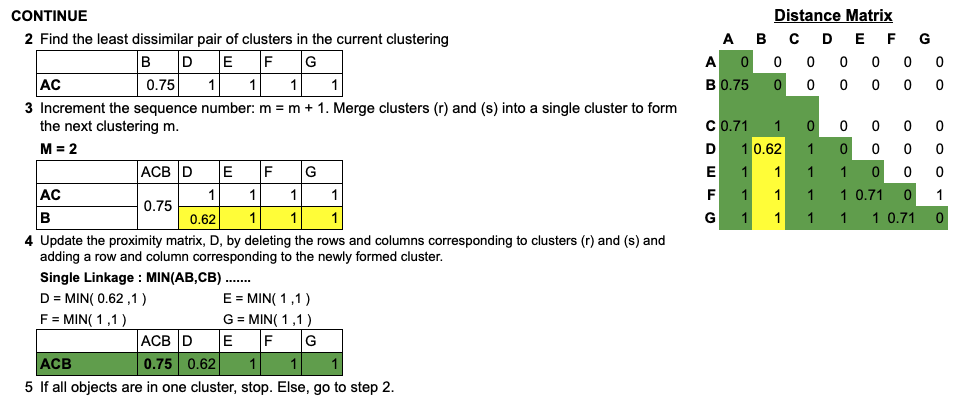
\includegraphics[width=14cm]{img/bab_3/hc_detail_2.png}
	\captionof{figure}{Lanjutan Proses Perhitungan \textit{Hierarchical Clustering}}
	\label{fig:hc_detail_2}
\end{center}

\begin{center}
	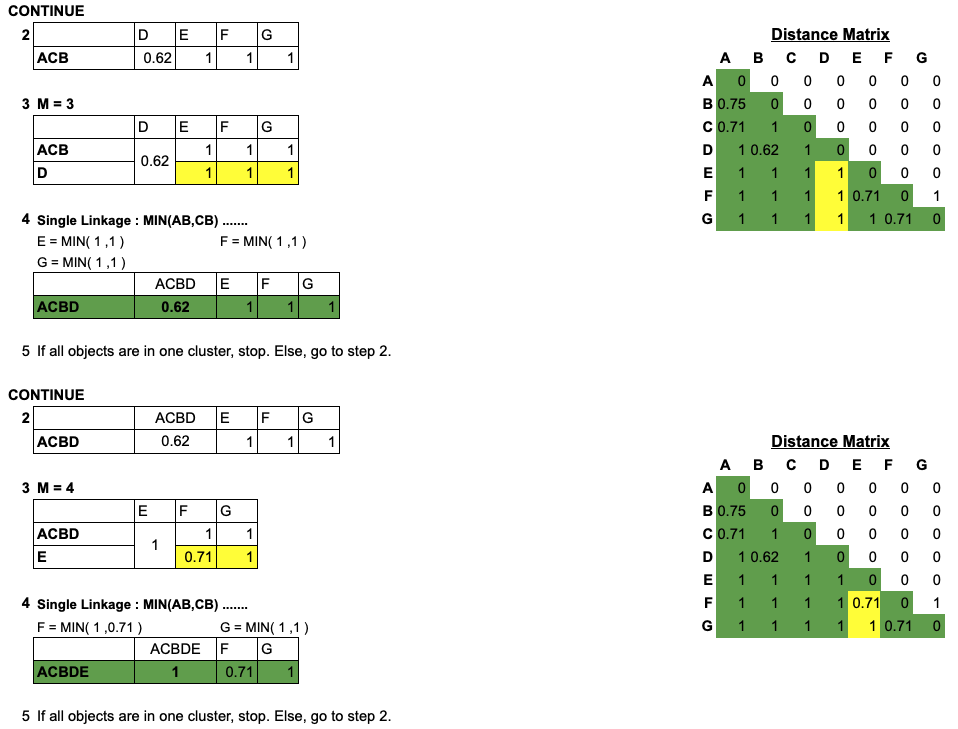
\includegraphics[width=14cm]{img/bab_3/hc_detail_3.png}
	\captionof{figure}{Lanjutan Proses Perhitungan \textit{Hierarchical Clustering}}
	\label{fig:hc_detail_3}
\end{center}

\begin{center}
	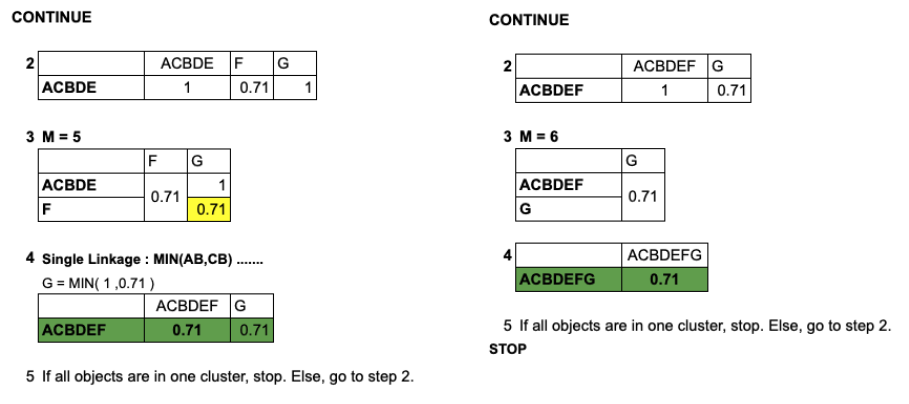
\includegraphics[width=14cm]{img/bab_3/hc_detail_4.png}
	\captionof{figure}{Lanjutan Proses Perhitungan \textit{Hierarchical Clustering}}
	\label{fig:hc_detail_4}
\end{center}

Hasil pengelompokan dapat ditampilkan dalam bentuk dendogram.  Di mana pengelompokan dari setiap \textit{linkage} memiliki dampak berbeda yang bisa dilihat dari bentuk dan nilai kedekatan antar partisi melalui dendogram dan bentuk relasi. Angka gabungan yang ditampilkan pada dendogram merupakan jarak \textit{linkage} yang dihitung dari proses perhitungan \textit{Hierarchical Clustering} sebelumnya.

\begin{center}
	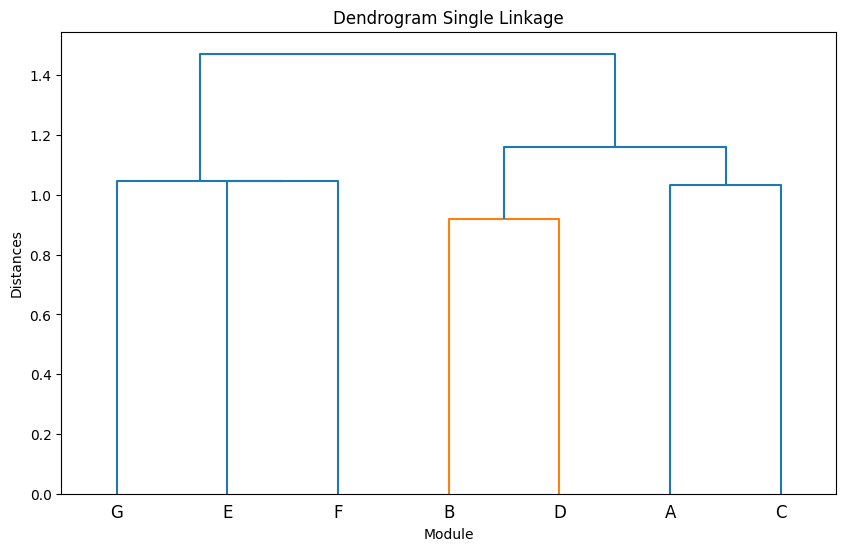
\includegraphics[width=11cm]{img/bab_3/singleLink.png}
	\captionof{figure}{Dendogram \textit{Single} \textit{Linkage}}
	\label{fig:asd}
\end{center}
\begin{center}
	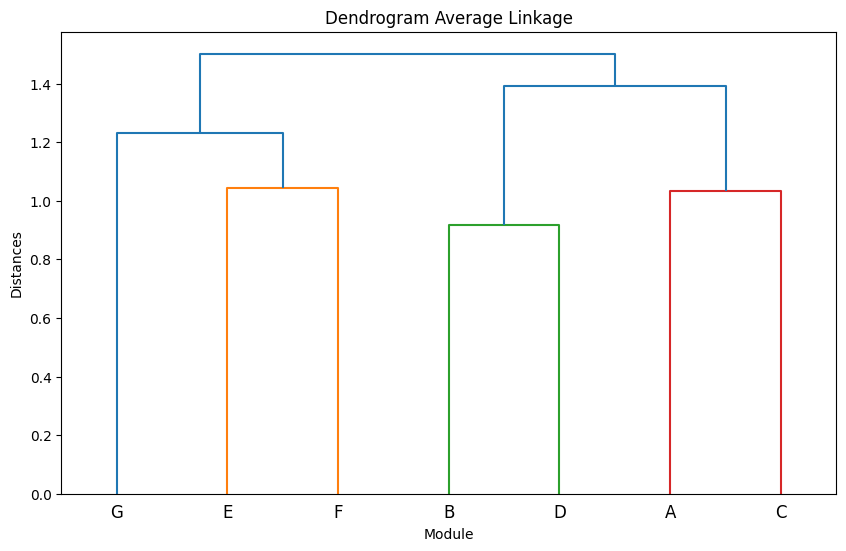
\includegraphics[width=11cm]{img/bab_3/averageLink.png}
	\captionof{figure}{Dendogram \textit{Average} \textit{Linkage}}
	\label{fig:asd}
\end{center}
\begin{center}
	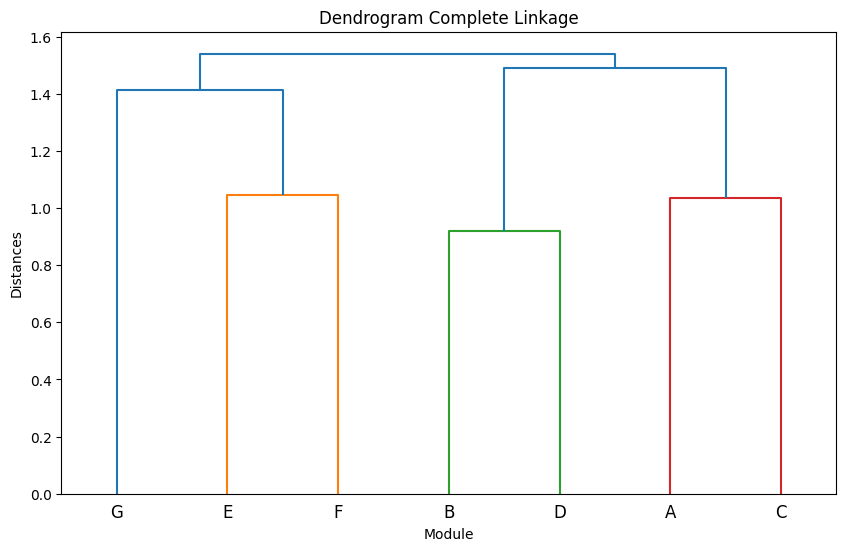
\includegraphics[width=11cm]{img/bab_3/completeLink.png}
	\captionof{figure}{Dendogram \textit{Complete} \textit{Linkage}}
	\label{fig:asd}
\end{center}

\subsubsection{Pemilihan Partisi}
Pemilihan jumlah partisi perlu dilakukan dengan perhitungan yang dapat menentukan jumlah \textit{service} yang ideal. \textit{Microservice} yang ideal memiliki nilai \textit{coupling} yang rendah dan nilai \textit{cohesion} yang tinggi. Untuk itu tugas akhir ini menentukan partisi dengan nilai struktural yang menggunakan persamaan 2.2 dan tidak memperhitungkan nilai \textit{coupling} external karena addons pada Odoo dibuat dengan framework Odoo. Hubungan module luar seperti library umumnya dilakukan oleh framework Odoo sendiri bukan oleh addons.

Untuk pemilihan partisi harus mempertimbangkan nilai \textit{cohesion}, nilai \textit{coupling}, jumlah \textit{service}, dan apakah \textit{service} tersebut seimbang. Partisi yang akan menjadi \textit{service} diharapkan bisa independen. 

Proses pemilihan partisi dimulai dari pemotongan tree dari hasil \textit{Hierarchical Clustering} sebelumnya. Pemotongan dilakukan berdasarkan jumlah cluster / partisi, kemudian  dipetakan dalam bentuk directed graph untuk menyusun kelompok partisi yang berisi relasi objek-objek / modul. Didalam node graph setiap hubungan module diluar dari partisinya akan dihitung sebagai panggilan ke luar dan hubungan antar module yang masih didalam  dihitung sebagai panggilan internal partisi.

\begin{center}
	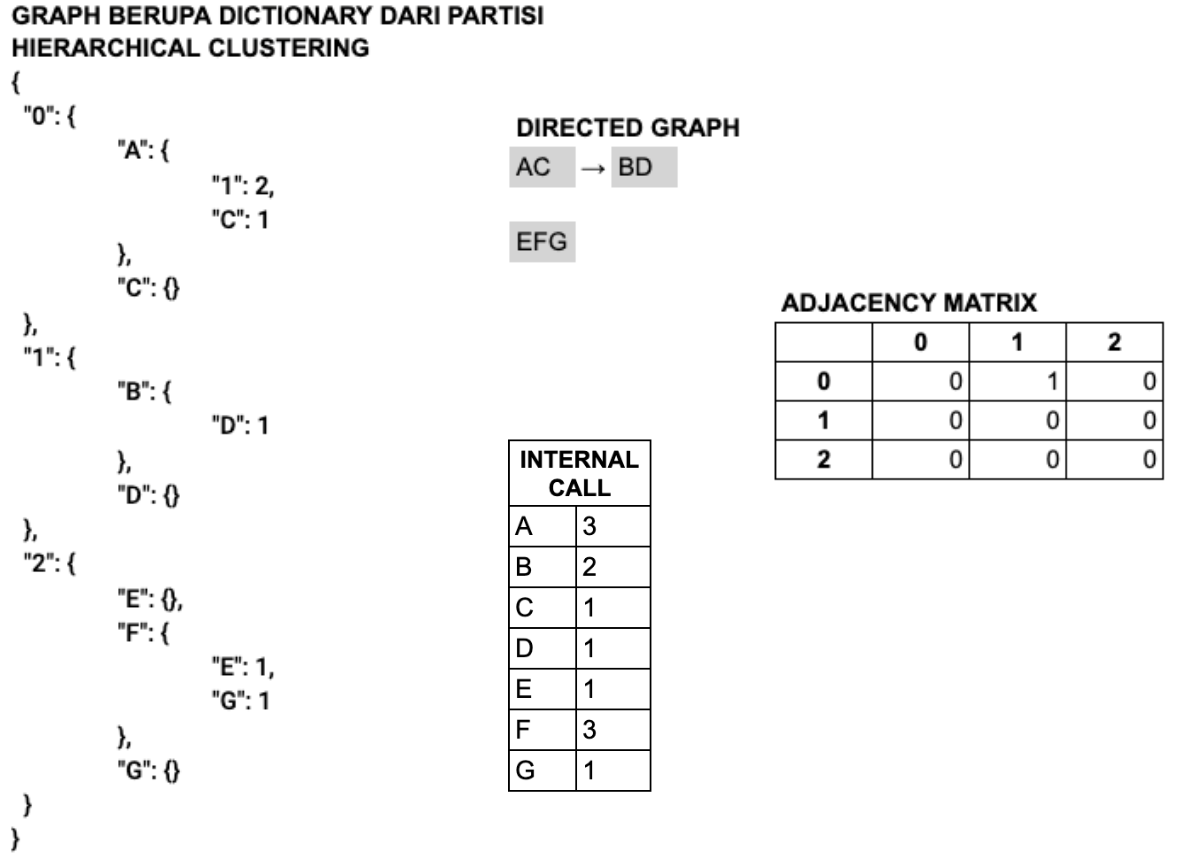
\includegraphics[width=14cm]{img/bab_3/eval_detail1.png}
	\captionof{figure}{Proses pemotongan tree dan perubahan menjadi \textit{Adjacency} \textit{Matrix}  dengan \textit{linkage} \textit{single} sejumlah 3 partisi}
	\label{fig:asd}
\end{center}

Module juga memiliki panggilannya internal masing-masing sebelumnya karena didalam module bisa berisi banyak sub-module lainnya, data ini disimpan dalam bentuk key-value dictionary. panggilan internal dibutuhkan untuk membuat kohesi yang benar dan panggilan eksternal (diluar partisi) digunakan untuk menghitung nilai coupling.  Pada tugas akhir ini menggunakan Structural and Behavioral Dependencies untuk mengevaluasi hasil partisi yang dihasilkan oleh \textit{Hierarchical Clustering}. Node graph diubah kembali menjadi \textit{Adjacency} \textit{Matrix} untuk memudahkan akses seperti komparasi hubungan antar partisi. 

\begin{center}
	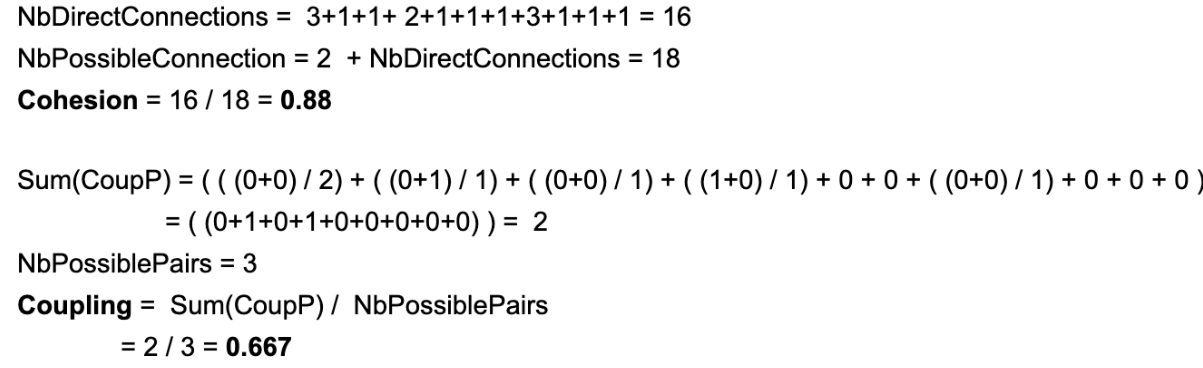
\includegraphics[width=14cm]{img/bab_3/eval_detail2.png}
	\captionof{figure}{Proses perhitungan coupling dan cohesion }
	\label{fig:asd}
\end{center}

Berikut adalah hasil nilai \textit{coupling} dan \textit{cohesion} masing-masing jumlah \textit{cluster}. Semakin tinggi jumlah \textit{cluster} maka nilai \textit{coupling} akan meningkat dan begitu pula sebaliknya untuk nilai \textit{cohesion}. Dari contoh data ditemukan bahwa \textit{cluster} yang ideal berjumlah 2 \textit{service}, karena ketika semakin banyak jumlah \textit{service} maka nilai \textit{coupling} meningkat dan sebaliknya nilai \textit{cohesion} menurun.


\begin{center}
	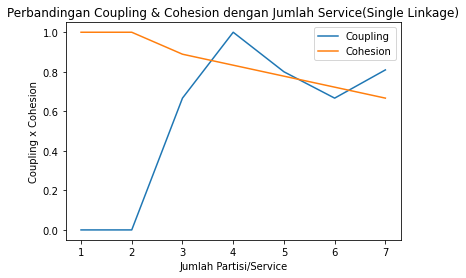
\includegraphics[width=12cm]{img/bab_3/cohVScoup_single.png}
	\captionof{figure}{Perbandingan dari nilai Cohesion dan nilai Coupling dengan jumlah \textit{cluster}/partisi menggunakan \textit{Single} \textit{Linkage}}
	\label{fig:asd}
\end{center}

\pagebreak

\subsection{Dekomposisi Monolitik ke \textit{Microservice}}
\subsubsection{Strategi Pemisahan Kode}
Odoo adalah aplikasi ERP berbasis web, tampilan pada Odoo bisa dibuka pada broser yang kompatibel. Odoo menggunakan pendekatan SPA (Single Page Application) dan adanya server rendering untuk menghasilkan HTML yang dinamik. Pada gambar \ref{fig:arsitektur_mono} terlihat bahwa aplikasi odoo merupakan aplikasi berbasis client-server.
\begin{center}
	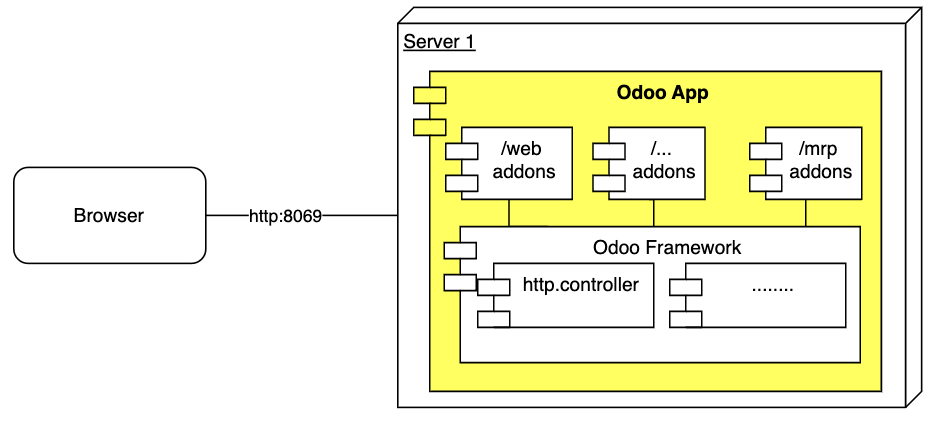
\includegraphics[width=12cm]{img/bab_3/mono_ori.png}
	\captionof{figure}{Arsitektur di Monolitik} 
	\label{fig:arsitektur_mono}
\end{center}

Proses pemisahan membutuhkan \textit{reverse} \textit{proxy} yang dapat menghubungkan client dengan banyak server. Tujuan adanya \textit{reverse} \textit{proxy} agar \textit{client} hanya perlu mengetahui satu pintu masuk aplikasi yaitu \textit{reverse} \textit{proxy} itu sendiri dan tidak perlu mengetahui seluruh server yang ada di aplikasi.

\begin{center}
	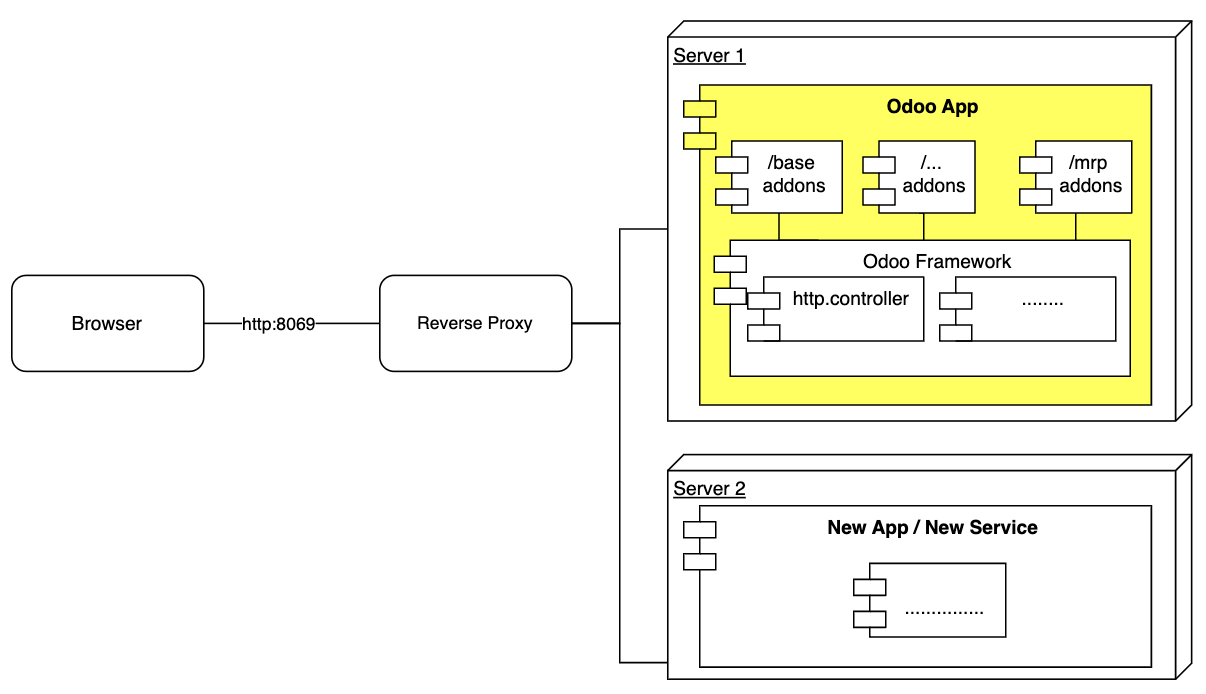
\includegraphics[width=14cm]{img/bab_3/micro_proxy.png}
	\captionof{figure}{Arsitektur di \textit{Microservice}}
	\label{fig:arsitektu_micro}
\end{center}

Berdasarkan landasan teori terdapat beberapa strategi pemisahan kode aplikasi monolitik, pada tugas akhir ini akan menggunakan 2 strategi yaitu pola \textit{Strangle} dan pola Branch by Abstraction. Pola \textit{Strangle} diterapkan karena pendekatan ini umum diterapkan dan lebih mudah pada suatu aplikasi yang sudah besar, dengan pola ini aplikasi monolitik bisa berdiri bersamaan dengan \textit{service} yang ingin dibangun atau dimigrasi. 

Tugas Akhir ini menggunakan \textit{API Gateway} Kong \textit{(off-the-shelf)} karena Kong sudah memiliki fitur yang lengkap pada kasus migrasi aplikasi monolitik ke \textit{microservice}. Fitur itu berupa kemampuan untuk redireksi url untuk menerapkan proses \textit{strangle}, pemantauan \textit{service}, dan memiliki performa yang baik.

\begin{center}
	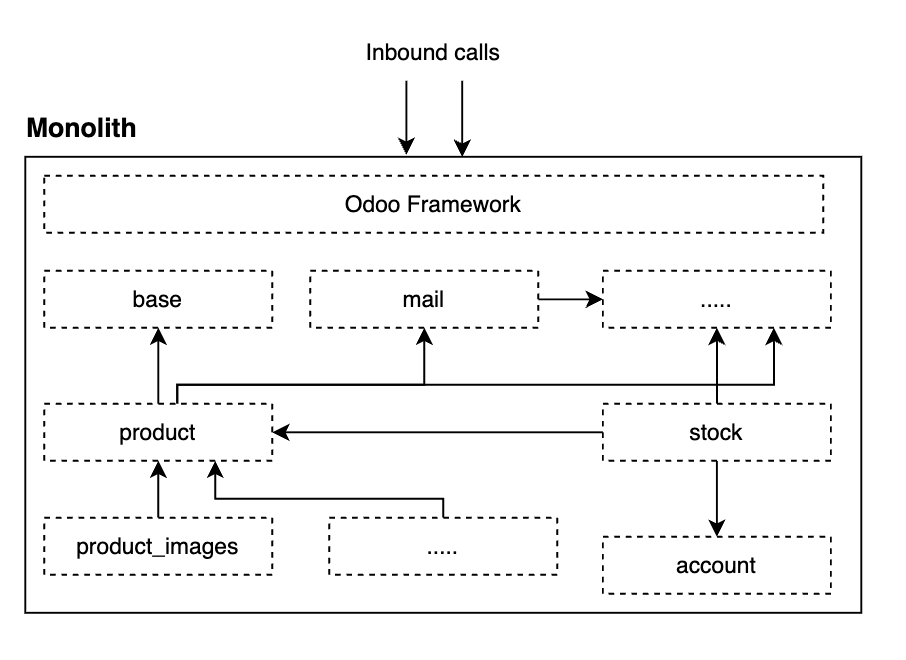
\includegraphics[width=10cm]{img/bab_3/strangelExMono.png}
	\captionof{figure}{Ilustrasi Struktur Module dan Keterhubungannya di Aplikasi Monolitik}
	\label{fig:asd}
\end{center}

Terdapat 3 langkah utama dalam menerapkan pola \textit{strangle} yaitu memilih bagian yang ingin dipindahkan, memindahkan aplikasi menjadi \textit{service} yang berdiri sendiri, dan yang terakhir mengubah \textit{call} dari monolitik ke \textit{service} yang baru dibuat.
 
Untuk menghubungkan antara bagian yang sudah dipisah dari monolitik dengan bagian yang masih di monolitik maka diperlukan penerapan pola Branch by Abstraction. Terdapat dua bagian utama yaitu abstract dan adapter. Abstract berperan menggantikan bagian yang sudah pisah menjadi \textit{service} sehingga bagian lain di monolitik tidak terdampak dan Adapter adalah implementasi sesungguhnya yang menghubungkan antara \textit{service} dan aplikasi monolitik.

\begin{center}
	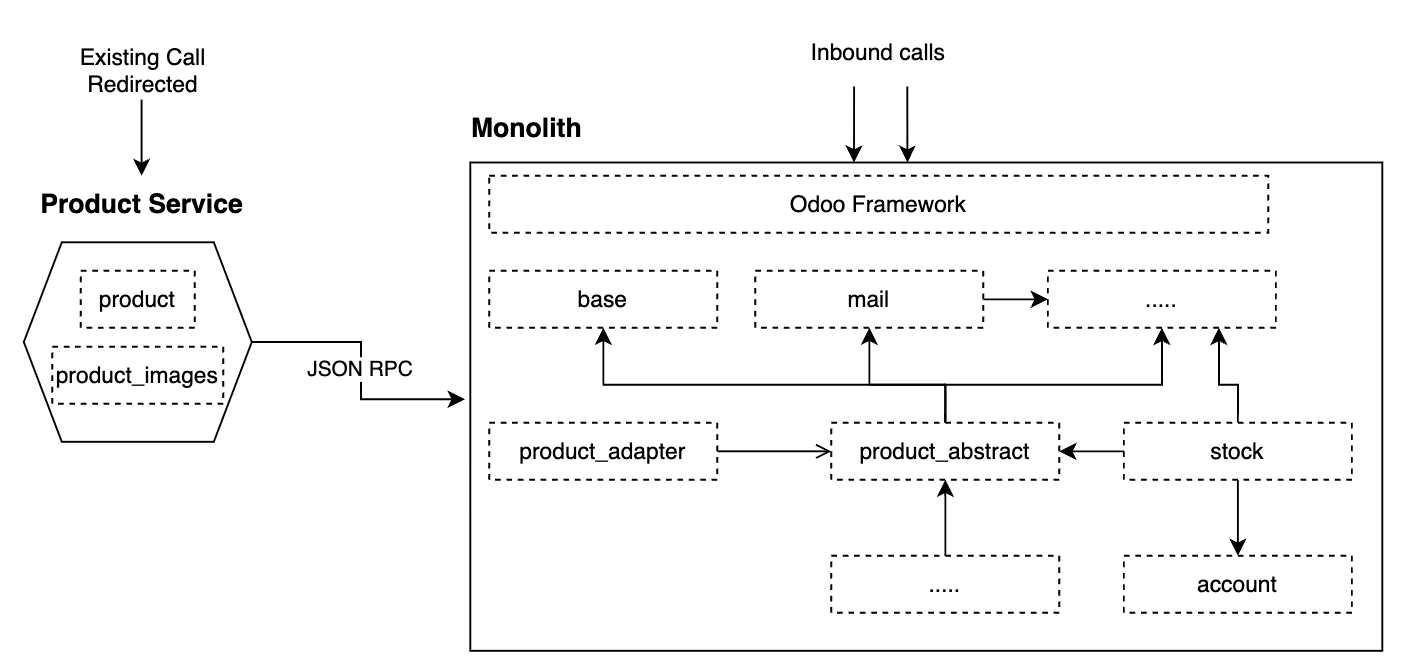
\includegraphics[width=12cm]{img/bab_3/strangelExMicro.png}
	\captionof{figure}{Penerapan Pola \textit{Strangle} dan Branch by Abstraction}
	\label{fig:asd}
\end{center}

Pemisahan kode mempengaruhi proses autentikasi, proses autentikasi pada aplikasi Odoo terdapat 2 cara yaitu melalui password atau API-Key. Odoo menyimpan sesi autentikasi di cookie namun bukan dalam format JSON Web Token (JWT) tapi bentuk HTTP session. Untuk itu diperlukan modifikasi pada sistem autentikasi yang menggunakan format JWT agar setiap \textit{service} tidak perlu menvalidasi berkali-kali apakah sesi itu valid. 

\begin{center}
	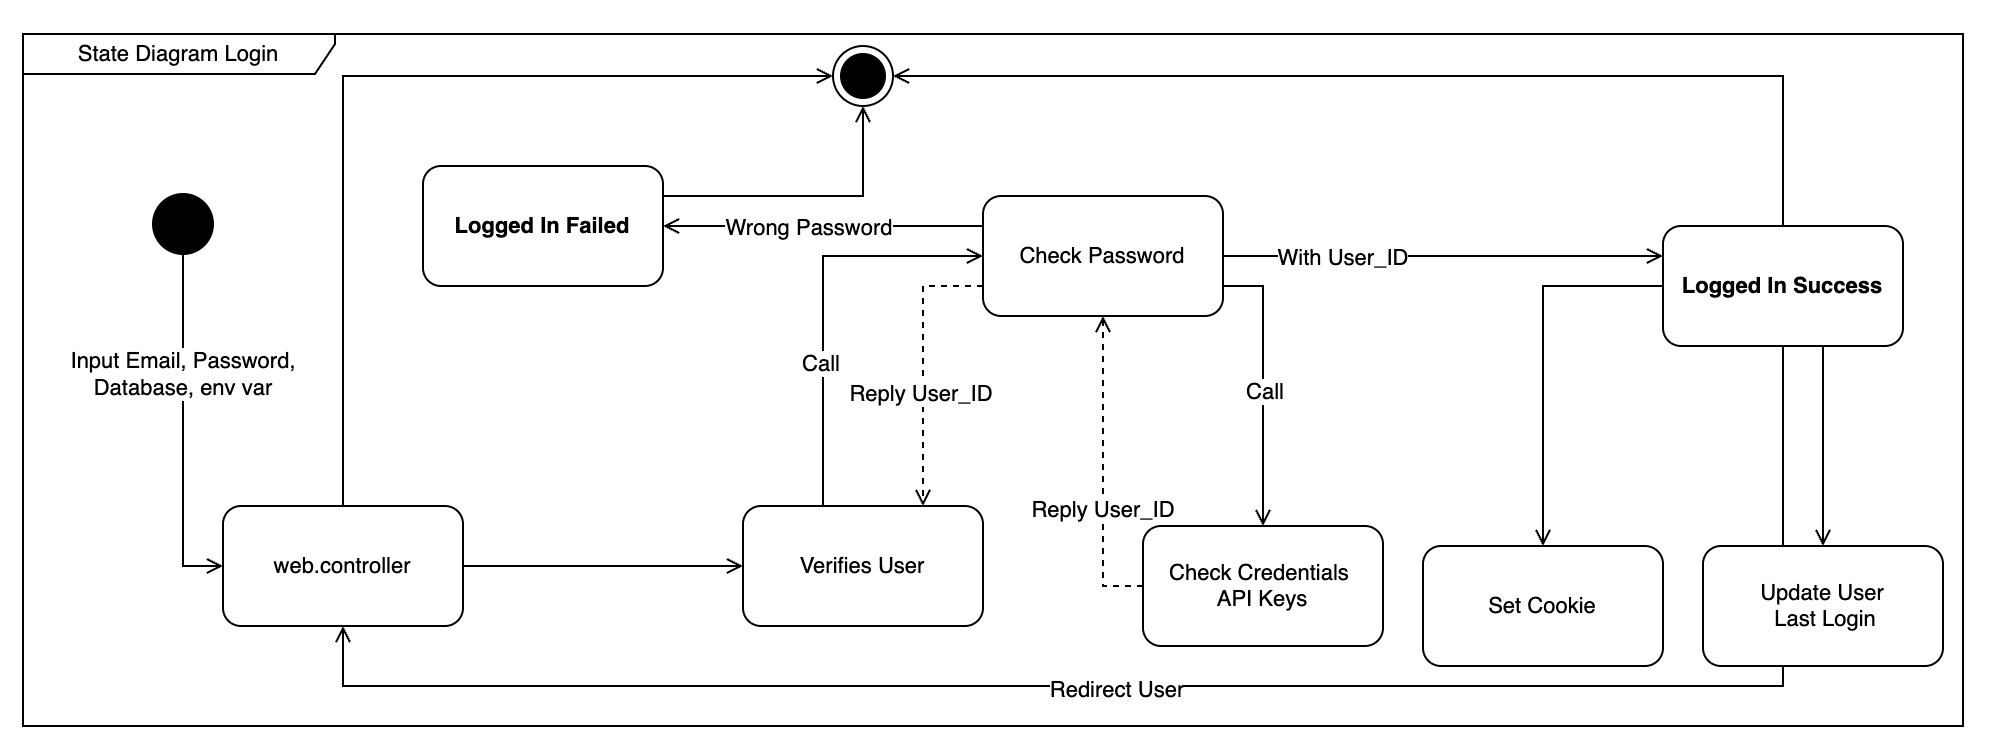
\includegraphics[width=14cm]{img/bab_3/stateDiagramLogin.png}
	\captionof{figure}{State Diagram pada proses login}
	\label{fig:asd}
\end{center}


\subsubsection{Komunikasi antar service}
Proses komunikasi antar \textit{service} dilakukan melalui JSON-RPC karena Odoo sudah memiliki untuk setiap addonsnya RPC ini bisa berupa XML atau JSON. Komunikasi ini melalui protokol  HTTP agar bisa akses oleh browser.  
\\
\subsubsection{Strategi Pemisahan \textit{database}}
Pemisahan \textit{database} dilakukan setelah dilakukan pemisahan kode karena pada Odoo sudah terdapat ORM yang mengelola \textit{database}. Ketika \textit{database} ingin dipisahkan maka pengaksesan \textit{database} monolitik  digunakan sebagai data access layer melalui API yang bisa berupa JSON-RPC.
\\ 

